%
%  PARA TRABALLOS EN GALLEGO USAR (LINEA 12): \usepackage[galician]{babel}
%  PARA TRABALLOS EN CASTELLANO USAR (LINEA 13): \usepackage[spanish]{babel}
%
% Para los acentos usamos codificacion UTF-8 (LINEA 10): \usepackage[utf8]{inputenc} 
% Si se usase la codificacion es_ES.ISO-8859-1 (LINEA 11): \usepackage[latin1]{inputenc}
% La conversion de acentos se hace con: iconv -f UTF-8 -t ISO-8859-1 filename.tex
%
% Como se incluyen figuras eps hay que compilar con: latex traballo , dvipdf traballo
%

\documentclass[12pt,twoside,a4paper]{book}
% pódense engadir todos os packages necesarios
\usepackage[utf8]{inputenc}
% \usepackage[latin1]{inputenc}
\usepackage[galician]{babel}
% \usepackage[spanish]{babel}
\usepackage{graphicx}
\usepackage[dvips]{epsfig}
\usepackage{amssymb}
\usepackage{eurosym}
\usepackage{float}
\usepackage{latexsym}
\usepackage{a4}
\usepackage{listings}
\usepackage{paralist}
\usepackage{parskip}
\usepackage[shortlabels]{enumitem}
\usepackage{hyperref}
\hypersetup{
    colorlinks,
    citecolor=black,
    filecolor=black,
    linkcolor=black,
    urlcolor=black
}
\setlength{\parindent}{1cm}
% \usepackage{hyperref} % menús no pdf pero non leva ben co package galician

\begin{document}
\pagestyle{empty}
\begin{center}
{\bf\Large UNIVERSIDADE DE SANTIAGO DE COMPOSTELA}

\vspace{0.5cm}

\includegraphics[width=5cm]{figuras/logo_usc.eps}

\vspace{0.5cm}
{\bf\large ESCOLA TÉCNICA SUPERIOR DE ENXEÑARÍA}

\vspace{2cm}
{\bf\LARGE Título do Traballo de Fin de Grao}

\vspace{0.5cm}
{\bf\LARGE Subtítulo do Traballo de Fin de Grao}
\end{center}

\vspace{2cm}
\hspace{4cm}\begin{tabular}{l}
{\it\Large Autor:} \\
{\bf\Large Pablo Pérez Romaní} \\
~ \\
{\it\Large Directores:} \\
{\bf\Large Paulo Félix Lamas} \\
{\bf\Large David González Márquez} \\
\end{tabular}

\vspace{2cm}
\begin{center}
{\bf\Large Grao en Enxeñaría Informática}

\vspace{0.5cm}
{\bf\large Setembro 2014}

\vspace{0.5cm}
Traballo de Fin de Grao presentado na Escola Técnica Superior de Enxeñaría da Universidade de Santiago de Compostela para a obtención do Grao en Enxeñaría Informática
\end{center}


\cleardoublepage
\pagestyle{plain}
\pagenumbering{roman}

\includegraphics[width=4cm]{figuras/logo_usc.eps}

\vspace{1cm}
{\bf D. Paulo Félix Lamas}, Profesor do Departamento de Electrónica e Computación da Universidade de Santiago de Compostela, e {\bf D. David González Márquez}, bolseiro de FPU do Centro de Investigación en Tecnoloxías da Información da USC,

\vspace{1cm}
INFORMAN:

\vspace{1cm}
Que a presente memoria, titulada {\it JDataMotion: unha ferramenta para a visualización dinámica de diagramas de dispersión}, presentada por {\bf D. Pablo Pérez Romaní} para superar os créditos correspondentes ao Traballo de Fin de Grao da titulación de Grao en Enxeñaría Informática, realizouse baixo nosa dirección no CiTIUS da Universidade de Santiago de Compostela.

\vspace{1cm}
E para que así conste aos efectos oportunos, expiden o presente informe en Santiago de Compostela, a 08/09/2014:

\vspace{2cm}
\begin{tabular}{lll}
Os codirectores, && O alumno, \\
~ \\
~ \\
~ \\
~ \\
~ \\
~ \\
~ \\
Paulo Félix Lamas & David González Márquez & Pablo Pérez Romaní
\end{tabular}

 % paxina de certificación (optativa)
%\cleardoublepage
% \pagestyle{plain}
\chapter*{Agradecementos}
Se se quere pór algún agradecemento, este vai aquí.

 % paxina de agradecementos (optativa) 
% \cleardoublepage
% \pagestyle{plain}
\chapter*{Resumo}
Se se quere pór resumo, este vai aquí.

 % páxina de resumo (optativa) 

\cleardoublepage
\pagestyle{plain}
\tableofcontents
\listoffigures
\listoftables

% Agora incluimos os capítulos. Cambiamos a numeración e as cabeceiras
\cleardoublepage
\pagenumbering{arabic}
\setcounter{page}{1}
\pagestyle{headings}
\chapter{Introdución}
\hyphenation{In-te-re-se}

Na actual sociedade da información, onde a cantidade de datos que se manexan aumenta día a día de xeito exponencial, a minería de datos convértese nunha ferramenta fundamental para poder explotalos de maneira eficaz, co fin último de xerar coñecemento a partir dos mesmos.

Para visualizar estes datos unha das técnicas máis utilizadas son os diagramas de dispersión ou scatterplots. Estes permítennos analizar os datos e atopar con facilidade relacións entre as distintas variables, como a correlación entre elas, a distribución dos puntos no plano, a tendencia dos datos recollidos ou outras características que sería complicado extraer a partir dun simple listado, posiblemente desordenado, de vectores de datos. Non obstante, os diagramas de dispersión restrínxennos a unha perspectiva estática do problema. En moitos deses problemas imos encontrar datos cunha compoñente que os sitúa no tempo. Con este proxecto pretendemos dotar a esta representación da súa perspectiva dinámica, para amosar os datos engadindo outro punto de vista que enriqueza a información extraida.

Deséxase desenvolver unha ferramenta para etiquetar cada punto dun diagrama de dispersión cun valor de significado temporal, de tal xeito que este puidese ser empregado como índice nunha visualización dinámica. Este valor numérico podería referenciar dende o momento de captación da tupla que a contén, ata unha ordenación dos datos atendendo á súa prioridade ou relevancia.

\section{Obxectivos xerais}

A motivación principal deste proxecto é o desenvolvemento dunha ferramenta capaz de visualizar a evolución dun conxunto de datos ao longo dunha magnitude como sería o tempo, ademais de permitir o preprocesado ou manipulación deses datos. Sendo máis específicos, este proxecto busca a realización da análise, deseño e implementación dunha aplicación que consiga: 

\begin{itemize}
\item Facilitarlle ao usuario o procesado de volumes de datos dun tamaño significativo. 
\item Posibilitar o traballo con formatos de arquivo CSV ou ARFF. 
\item Dispor das funcionalidades necesarias para manipular os datos. 
\item Ser capaz de amosar os datos en forma de diagramas de dispersión, con funcións de reprodución básicas. Tamén se debe posibilitar a configuración desta reprodución por parte do usuario. 
\item Aplicar filtros nos datos cos que se traballa, de xeito que se poidan eliminar datos fora dun rango, normalizar os seus valores, etc.
\item Interaccionar co usuario por medio dunha interface simple e amigable.
\item Aplicar nun caso real a ferramenta JDataMotion, para apreciar a súa utilidade.
\item Finalizar o desenvolvemento do proxecto antes do día 10 de Xullo de 2015.
\end{itemize} 

\section{Relación da documentación}

Esta memoria plasma o proceso de desenvolvemento do proxecto JDataMotion, que persegue os obxectivos citados no apartado anterior.

Os distintos capítulos repártense do modo que segue:

\begin{description}
\item[Capítulo 1. Introdución:] composta por obxectivos xerais, relación da documentación que conforma a memoria, descrición do sistema (métodos, técnicas ou arquitecturas utilizadas e xustificación da súa elección).
\item[Capítulo 2. Planificación e presupostos:] inclúe a estimación dos recursos necesarios para desenvolver este proxecto, xunto co custo (presuposto) e planificación temporal do mesmo, así como a súa división en fases e tarefas.
\item[Capítulo 3. Especificación de requisitos:] inclúe a especificación do sistema, xunto coa información que este debe almacenar e as interfaces con outros sistemas, sexan hardware ou software, e outros requisitos (rendemento, seguridade, etc).
\item[Capítulo 4. Deseño:] rexistra como se realiza o sistema, a división deste en diferentes compoñentes e a comunicación entre eles. Así mesmo, neste apartado determínase o equipamento hardware e software necesario.
\item[Capítulo 5. Exemplos:] Avaliación do grao de cumprimento dos requisitos e tests os verifican.
\item[Capítulo 6. Conclusións e posibles ampliacións.]
\item[Apéndice A. Manuais técnicos:] incluirase toda a información precisa para aquelas persoas que se vaian a encargar do desenvolvemento e/ou modificación do sistema.
\item[Apéndice B. Manuais de usuario:] incluirán toda a información precisa para aquelas persoas que utilicen o sistema: instalación, utilización, configuración, mensaxes de erro, etc.
\item[Apéndice C. Licenza.]
\item[Bibliografía]
\end{description} 
\cleardoublepage
\chapter{Xestión do proxecto}

Neste capítulo comentaremos distintos aspectos relacionados coa planificación de como se vai xestionar este proxecto. Falaremos, por exemplo, da xestión de riscos que conleva o desenvolvemento do software, así coma os métodos de continxencia, prevención ou minimización que seguiremos en caso da incidencia dos mesmos. Cos riscos expostos, abordaremos a metodoloxía de desenvolvemento máis axeitada para o proxecto, de acordo tamén cos obxectivos anteriormente plasmados. Seguiremos coa planificación temporal do proxecto e finalizaremos coa estimación de custo e prazos, así como a xestión da configuración. 

\section{Xestión de riscos}

Na fase de planificación dun proxecto hai que sopesar os distintos riscos aos que estará exposto o seu desenvolvemento, cuantificalos e deseñar estratexias para a súa aparición. Algúns dos riscos nun Traballo de Fin de Grao poden ter graves consecuencias na liña base do proxecto debido á inexperiencia do seu autor, polo que fronte á falta de experiencia hai que esforzarse en mellorar a planificación.

No análise de riscos valoraremos a probabilidade de aparición e a súa gravidade, para a continuación deseñar unha medida de continxencia, prevención ou minimización. A escala de valoración da probabilidade e da gravidade vai ser:

\begin{itemize}
\item Moi baixa
\item Baixa
\item Media
\item Alta
\item Moi alta
\end{itemize} 

Os riscos considerados son os seguintes:

\begin{itemize}

\item \textbf{Risco 01}
\begin{description}
\item[Nome:] Cambios no alcance durante o desenvolvemento
\item[Descrición:] A lista inicial de requisitos funcionais que se captará nas primeiras reunións cos titores vai sufrir modificacións, incluso co proxecto en etapas avanzadas de desenvolvemento. A súa probabilidade duplícase pola dobre titularidade do Traballo de Fin de Grao.
\item[Probabilidade:] Moi alta
\item[Gravidade:] Alta
\item[Medidas de minimización:] Botaremos man da folgura temporal do proxecto (marxe de tempo dispoñible para eventualidades). Os cambios razoaranse cos titores, presentando a lista de requisitos actual e valorando a parte da folgura que consumirían ditos cambios. Tamén se tratará de ter reunións de avaliación cos titores cunha alta frecuencia, para así detectar o antes posible calquera cambio nos requisitos, se ben pode acontecer que se propoñan cambios sobre as primeiras etapas cando o proxecto se atopa en etapas avanzadas.
\end{description}

\item \textbf{Risco 02}
\begin{description}
\item[Nome:] Confrontación de opinións entre os distintos titores
\item[Descrición:] Un cambio ou opinión dun titor contradí á do outro.
\item[Probabilidade:] Moi alta
\item[Gravidade:] Media
\item[Medidas de prevención:] Trataremos de citarnos cos dous titores á vez, de xeito que calquera dualidade de opinións se resolva de xeito presencial. Nestes casos o risco non será considerado como acontecido.
\item[Medidas de minimziación:] Cando as reunións non se podan realizar cos dous titores á vez, informarase ao outro o antes posible das decisións, acordos ou cambios prantexados, así poderemos coñecer a súa opinión antes de obrar en consecuencia. Intentarase que toda esta comunicación externa ás reunións se realice por correo electrónico, e tratarase de incluír a todos os participantes (menos ao propio emisor) no grupo de destinatarios das mensaxes. Ademais, deste xeito quedará rexistrada a resposta e evitarase o repudio.
\end{description}

\item \textbf{Risco 03}
\begin{description}
\item[Nome:] Imprecisión á hora de fixar entregables
\item[Descrición:] A inexperiencia do alumno manifestarase xa nas primeiras entregas programadas. Ao non ter traballado previamente en proxectos desta índole, resultará complicado estimar os prazos de entrega nas primeiras fases do proxecto, tanto por exceso como por defecto.
\item[Probabilidade:] Alta
\item[Gravidade:] Media
\item[Medidas de minimización:] Intentaremos especificar entregas dun contido menor e máis frecuentes, sobre todo nas primeiras fases, para que sexa máis doado comezar a estimar correctamente os prazos de entrega.
\end{description}

\item \textbf{Risco 04}
\begin{description}
\item[Nome:] Imposibilidade de reunirse cun dos titores
\item[Descrición:] Un dos titores non pode acudir a algunha reunión proposta, nin estará nos seguintes 5 días.
\item[Probabilidade:] Alta
\item[Gravidade:] Baixa
\item[Medidas de minimización:] Desenvolverase a reunión co titor dispoñible, sendo mester, de acordo co Risco 02, informar das conclusións sacadas ao outro titor por medio do correo electrónico en canto remate a reunión.
\end{description}

\item \textbf{Risco 05}
\begin{description}
\item[Nome:] Imposibilidade de reunirse con ningún dos dous titores
\item[Descrición:] Ningún dos titores está dispoñible para unha reunión, nin estará nos seguintes 5 días.
\item[Probabilidade:] Media
\item[Gravidade:] Media
\item[Medidas de minimización:] Tratarase de programar unha videoconferencia con polo menos un dos dous titores. No caso dun só titor, abordaranse as medidas adoptadas para o Risco 4. Se isto non fose posible, continuaríase traballando no seguinte entregable ata que algún dos titores volvese estar dispoñible.
\end{description}

\item \textbf{Risco 06}
\begin{description}
\item[Nome:] Descoñecemento ou inexperiencia coas solucións
\item[Descrición:] O alumno non coñece as posibilidades que teñen as ferramentas das que dispón (librarías, módulos, solucións, etc.).
\item[Probabilidade:] Alta
\item[Gravidade:] Media
\item[Medidas de prevención:] Adicarase un tempo prudencial, nas primeiras fases, a revisar as APIs e a documentación en xeral das librerías, proxectos de terceiros e demais ferramentas que se van empregar, para ser conscientes de como poden solucionar as nosas necesidades.
\end{description}

\item \textbf{Risco 07}
\begin{description}
\item[Nome:] Mala escalabilidade do sistema
\item[Descrición:] O noso sistema escala mal con entradas de datos de gran tamaño.
\item[Probabilidade:] Alta
\item[Gravidade:] Media
\item[Medidas de minimización:] Programaremos prazos de tempo maiores para entregas nas que a escalabilidade poida ser un problema (visualización, carga de datos, etc.) para mellorar este aspecto. Se non é viable reducir máis a latencia, procederase a aliviala mellorando a usabilidade do sistema (por exemplo, empregando barras de progreso).
\end{description}

\item \textbf{Risco 08}
\begin{description}
\item[Nome:] Imposibilidade de finalizar o proxecto en tempo
\item[Descrición:] A folgura está esgotada, e o cumprimento do prazo de entrega vese ameazado.
\item[Probabilidade:] Media
\item[Gravidade:] Moi alta
\item[Medidas de prevención:] Evitaremos na medida do posible recorrer á folgura, e trataremos de seguir a planificación do xeito máis estrito que podamos.
\item[Medidas de minimización:] Poremos en coñecemento aos titores do estado do proxecto e dos seus prazos, para discutir a modificación ou eliminación dalgúns ítems da especificación.
\end{description}

\end{itemize}

\section{Metodoloxía de desenvolvemento}

A elección da metodoloxía de traballo é un paso importante na planificación de calquera proxecto, xa que a posteriori influirá en varios aspectos deste: a xestión dos seus riscos, a súa tolerancia a cambios externos, a confianza na súa validez, etc. Hai dous enfoques fundamentais: as metodoloxías estritas e as metodoloxías áxiles. As primeiras esixen unha planificación estrita, practicamente inmutable e necesariamente realista de todo o plan de traballo, e son boas cando o conxunto de requisitos é fixo e moi concreto. As segundas, pola contra, son flexibles e adáptanse ben a cada situación, pois nelas asúmese que se van producir variabilidades nos requisitos.

Sopesando as circunstancias nas que se desenvolve un Traballo de Fin de Grao, onde a experiencia do alumno é practicamente nula no que respecta a xestión de proxectos, e tendo en consideración dous clientes (titores) aos que atender, semella que deberíamos adoptar unha metodoloxía de traballo que se adapte ás necesidades de cambios que vaian xurdindo, e que consiga en cada entrega recibir certo 'feedback' por parte dos titores, de forma que tras cada iteración podamos ter a seguridade da correspondencia entre o proxecto e o modelo mental de quen o especificou. É dicir, necesitamos unha metodoloxía áxil.

Dentro do compendio de metodoloxías áxiles existentes, decantarémonos pola metodoloxía Scrum\cite{scrum}, pois enfoca todas as súas avaliacións sobre entregas parciais, pero funcionais, para facilitarlle ao receptor do proxecto a valoración do mesmo. Necesítase, polo tanto, unha gran implicación do cliente no proxecto, algo que se pode conseguir dada a dualidade da titoría (é máis doado que haxa un titor dispoñible para realizar a reunión). Por outra banda, os requisitos que constitúen as distintas entregas deben estar priorizados para que o proxecto poida avanzar cun carácter incremental, e ditas entregas deben resultar usables para o cliente.

Scrum define unha serie de ferramentas e de regras, idóneas para levar a cabo o desenvolvemento de proxectos que buscan unha metodoloxía áxil. Os preceptos básicos deste modelo son:

\begin{itemize}
\item Adoptar unha estratexia de desenvolvemento incremental, no canto da planificación e execución completa do produto (é dicir, no canto dunha metodoloxía estrita).
\item Basear a calidade do resultado máis no coñecemento das persoas que o especificaron ca na calidade dos procesos empregados.
\item Solapamento das fases de desenvolvemento (análise, deseño, implementación e probas) no canto da sucesión secuencial que nos ofrecen metodoloxías como a cascada.
\end{itemize} 

A metodoloxía Scrum comeza cunha captación de requisitos en reunión co cliente, da cal se extrae un Backlog, é dicir, unha lista ordenada por prioridade de requisitos funcionais (RFs). Ademais, Scrum define o sprint como unidade elemental de tempo de traballo. Un sprint dura entre 1 e 4 semanas, aínda que nós trataremos de manter a súa duración en 2 ou incluso 1 semanas para maximizar a supervisión e xestionar ben os riscos, sobre todo nas etapas iniciais.

Ao término de cada reunión co cliente, revísase o Backlog e incorpórase un certo número de RFs a un novo sprint, o cal dará comezo en canto remate a reunión. Para o remate dese novo sprint (dentro dunha semana no noso caso) terase programada a seguinte reunión, na que se valorará o sprint finalizado e se accederá ao Backlog para acordar o seguinte sprint, e así sucesivamente. A valoración do sprint en cada reunión realízase presentando a lista de RFs de dito sprint, e demostrando ante o receptor do proxecto que cada un dos ítems ou tarefas do sprint funciona correctamente.

Para regular o desenvolvemento desa metodoloxía pódese botar man de diversas ferramentas, de entre as cales nós escollemos Acunote\cite{acunote} para o noso proxecto. Acunote é unha aplicación web especialmente deseñada para a xestión da metodoloxía Scrum. Ten varios plans de prezos, pero nós empregaremos o gratuíto porque as nosas necesidades restrínxense a un equipo de persoal pequeno (o alumno e os dous titores). Entre as prestacións desta ferramenta, sacarémoslle maior proveito ás seguintes:

\begin{description}
\item[Wiki:] Empregarémola para engadir contido visible ao resto de membros do grupo.
\item[Lista de sprints:] Amosa os sprints en 3 grupos: sprints pasados, sprints presentes e sprints futuros. Ao abrir un sprint visualízanse os ítems ou tarefas (requisitos funcionais no noso caso) que o compoñen. Accederemos a este apartado na maioría dos casos para crear novos sprints.
\item[Sprint actual:] Visualiza os RFs do sprint actual. A medida que se vaian completando requisitos funcionais, accederase a esta lapela para cambiar o estado do requisito en cuestión. Os estados posibles son:
\begin{itemize}
\item Non comezado (por defecto)
\item En progreso
\item Reaberto
\item Bloqueado
\item Completado
\item Verificado
\item Duplicado
\item Non se vai realizar
\end{itemize}
\item[Backlog:] Contén todos os ítems (requisitos funcionais) pendentes de ser asignados a un sprint. Este lista cumprimentarase ao principio, cos requisitos funcionais captados e ordenados por prioridade, e logo accederase a ela á hora de asignar RFs aos novos sprints. Na extracción de RFs débese respectar a orde dos mesmos dentro da lista, collendo sempre un número de ítems determinado da parte superior. Estes ítems desaparecerán do Backlog en canto sexan asignados.
\item[Tarefas:] Mostra todos os ítems especificados, independentemente de que fosen asignados a un sprint ou non.
\end{description} 

\section{Planificación temporal}

A metodoloxía Scrum caracterízase como ben dixemos polo solapamento das fases que nun modelo en cascada estarían ben separadas. As primeiras semanas de traballo estarán adicadas á análise para a captación inicial de requisitos, pero nas sucesivas iteracións ou sprints poderán realizarse en paralelo análise, deseño, implementación e probas. Esta é unha das licencias que outorga o emprego das metodoloxías áxiles. De todos xeitos, aínda dentro da variabilidade destas metodoloxías, podemos dividir a vida do proxecto en unha serie de fases fundamentais:
\begin{description}
\item[Inicio:] Constitúe o primeiro sprint (Sprint 00) da planificación, e durará dúas semanas. Nesta fase programaranse reunións cos titores para realizar a captación de requisitos funcionais (análise de requisitos), e ordenaranse estes por prioridade, dando lugar ao Backlog. Tamén se definirá a especificación de cada requisito e se deseñarán as proba que os verifiquen.
\item[Desenvolvemento:] Abrangue dende o Sprint 01 ata o Sprint 11, ambos inclusive (20 semanas en total). Nesta fase elaborarase o produto de acordo cos requisitos
\item[Documentación:] Abrangue 5 semanas de traballo. Nesta fase recompilarase toda a documentación xerada nas fases anteriores, e confeccionarase a memoria e máis a presentación, que constituirán os entregables do Traballo de Fin de Grao.
\end{description}

En total, o proxecto traballarase durante un período de 27 semanas (189 días, algo máis de 6 meses), co cal, para realizar as 401,25 horas de traballo necesarias teremos que levar un ritmo de traballo aproximado de 15,28 horas semanais (unha media de 2 horas e cuarto diarias). Non nos convén asumir un ritmo de traballo maior, pois durante ese período de tempo o alumno deberá repartir a súa axenda entre este proxecto, o resto de materias, as prácticas en empresa, etc.

A continuación e en base ao especificado no anteproxecto (sprints e planificación temporal dos mesmos), exporemos na Figura \ref{gantt} o Diagrama de Gantt que ilustra a planificación temporal das fases. Cómpre destacar que a fase de Desenvolvemento será dividida nos sprints que a compoñen directamente.

\begin{figure}
\centering
\includegraphics[width=\textwidth,height=\textheight,keepaspectratio]{figuras/gantt}
\caption{Diagrama de Gantt}
\label{gantt}
\end{figure}

Do mesmo xeito, coa referencia do anteproxecto extraemos na Figura \ref{edt} o Esquema de Descomposición do Traballo (EDT) do proxecto. Cada fase anterior amosarase dividida nas tarefas que a compoñen. Cabe destacar que na fase de Desenvolvemento, para cada sprint, as tarefas que ten asignadas son os propios requisitos funcionais (RFs) a implementar nese sprint, ou o que é o mesmo, a implementación de cada RF constitúe a tarefa que o representa. Por exemplo, o RF 'Insertar filtros' impleméntase na tarefa do mesmo nome: Insertar filtros.

\begin{figure}
\centering
\includegraphics[width=\textwidth,height=\textheight,keepaspectratio]{figuras/edt}
\caption{Esquema de Descomposición do Traballo (EDT)}
\label{edt}
\end{figure}

\section{Xestión da configuración}

Todo proxecto ten elementos de interese para incluír na xestión da configuración. Estes elementos caracterízanse porque son candidatos a sufrir cambios que poden ameazar o correcto desenvolvemento do proxecto. A xestión da configuración trata de manter a integridade do proxecto perante a estes cambios. O noso deber é identificar que obxectos do proxecto (sexan entregables ou resultados parciais do mesmo) merecen a súa inclusión na xestión da configuración, e por outra parte, temos que especificar que ferramentas empregaremos para dar soporte a esta característica.

Para este caso consideraremos ao código fonte do proxecto (e máis das súas probas) e á documentación como elementos de configuración, que se corresponden coas carpetas 'src', 'test' e 'doc' respectivamente. O código fonte é o sustento do noso proxecto, e os cambios no seu contido veranse directamente reflexados no produto a entregar, polo que é mester incluír este elemento na xestión da configuración. Tamén incluiremos o código fonte das probas porque debemos respectar a integridade entre estas e o propio proxecto. Por outra parte, a documentación sufrirá cambios de xeito paralelo ao código, e evolucionará da man deste ao longo da vida do proxecto (rexistrará a súa especificación de requisitos, o seu deseño, etc.), así que tamén debe ser un elemento a considerar en aras de preservar a integridade do proxecto. En resumo, faremos seguimento de cambios dos tres directorios ('src', 'test' e 'doc'), e para iso botaremos man do software GitHub\cite{github}.

Github é unha forxa para darlle aloxamento a distintos tipos de proxectos, por medio do sistema de control de versións Git. Para aloxar o noso proxecto crearemos un repositorio local e outro remoto, chamando a ambos 'JDataMotion', e outorgándolle ao remoto permisos de lectura e escritura para o alumno e permisos de lectura (ou de escritura tamén, opcionalmente) para os titores. Deste xeito estes poderán descargar a última versión do proxecto en calquera momento, mentres que o alumno poderá ir facendo '{\it pushes}' cada certo tempo cos cambios implementados.

O proxecto conten moitos máis elementos, pero non podemos consideralos a todos aptos para a xestión de configuración por diversos motivos: as librarías empregadas (directorio 'lib') non cambian (e no caso de querer actualizar algunha, asúmese que non deben xurdir problemas de integridade gracias á compatibilidade entre versións), e os ficheiros de código obxecto e de distribución ('build' e 'dist') dependen directamente do código fonte (que xa é un elemento de configuración), pois xéranse como resultado da súa compilación.

\section{Análise de custos}

A estimación dos custos de desenvolvemento do proxecto amósase no Cadro \ref{tab:custosLabel}. Para ela, consideramos a adquisición dun novo equipo informático. As horas de traballo neste caso non van ter un valor económico asociado, como consecuencia de que este proxecto pertenza a un Traballo de Fin de Grao, pois as horas do traballo do alumno correspóndense coas que este debe cumprimentar para a obtención do título. Para o consumo eléctrico tivemos en conta o prezo do kWh en España\cite{preciokWh_espana} e fixemos unha estimación\cite{energyusecalculator} do consumo en Watios dun equipo informático, que a plena potencia pode traballar a 120 vatios. Considerando que o desenvolvemento  do traballo durará 401.25 horas, necesitaremos 120 W * 401.25 h = 48150 Wh = 48,15 kWh. Ademais, tratarase sempre de buscar solucións 'freeware' ou de software gratuíto ás distintas necesidades de módulos adicionais que vaian xurdindo, polo que o custo económico destas será nulo.

% Table generated by Excel2LaTeX from sheet 'Hoja1'
\begin{table}[htbp]
  \centering
    \begin{tabular}{rrrrr}
    \textbf{Activo} & \textbf{Cantidade} & \textbf{C.U. sen IVE} & \textbf{IVE} & \textbf{Custo total} \\
    Ordenador portátil & 1     & 570,00 \euro & 21\%  & 689,70 \euro \\
    Horas de traballo & 401,25 horas & 0,00 \euro/hora & 21\%  & 0,00 \euro \\
    Consumo eléctrico & 48,15 kWh & 0,12 \euro/kWh & 21\%  & 7,23 \euro \\
          &       &       & \textbf{Total} & 696,93 \euro \\
    \end{tabular}%
		\caption{Custos}
  \label{tab:custosLabel}%
\end{table}%


\cleardoublepage
\chapter{Análise de requisitos}

A extracción dos requisitos dun proxecto é unha fase fundamental na realización de calquera proxecto, pois inflúe non só nas propias tarefas a desenvolver para a súa implementación, se non tamén na valoración do produto final e da súa calidade. A obtención de requisitos adóitase facer durante ou tras unha reunión co cliente.

\section{Casos de uso}

Os casos de uso empréganse para modelar e representar nun primeiro momento cómo se vai realizar a interacción entre o sistema e os usuarios del, tamén coñecidos como actores. Os casos de uso constitúen as posibilidades das que dispón cada actor. Este análise resulta especialmente útil en entornas orientadas a usuarios con distinta prioridade (un administrador, un usuario invitado, un usuario rexistrado, un usuario prémium, etc.) nas que cada un deses actores ten acceso a uns casos de uso específicos (por exemplo, moitas aplicacións web). Por tanto, a riqueza dos diagramas de casos de uso radica na variedade de tipos de usuario (actores). A nosa aplicación non necesita facer distinción algunha entre os tipos de usuario que poden facer uso dela. Todos van dispor das mesmas funcionalidades. En conclusión, o diagrama de casos de uso non aportaría ningunha información nova, así que será omitido.

\section{Requisitos funcionais}

\subsection*{RF01}
\begin{description}
\item[Título] \hfill \\
Importar arquivos con datos para o experimento
\item[Descrición] \hfill \\
A aplicación debe permitir cargar do sistema de arquivos un ficheiro que conteña unha secuencia de datos (nun formato axeitado segundo o RNF02) para ser utilizados no experimento.
\item[Casos de uso relacionados] \hfill \\
\item[Importancia] \hfill \\
Esencial
\end{description}

\subsection*{RF02}
\begin{description}
\item[Título] \hfill \\
Exportar datos
\item[Descrición] \hfill \\
A aplicación debe permitir almacenar nun arquivo o conxunto de datos do arquivo actual (tendo en conta filtrados, modificacións, datos engadidos ou eliminados...). Os arquivos de saída deben respectar o RNF02.
\subsubsection{Importancia}
Esencial
\end{description}

\subsection*{RF03}
\begin{description}
\item[Título] \hfill \\
Gardar sesión
\item[Descrición] \hfill \\
A aplicación debe permitir gardar en disco a sesión (ou experimento) actual tal e como está no momento de executar esta acción.
\item[Importancia] \hfill \\
Esencial
\end{description}

\subsection*{RF04}
\begin{description}
\item[Título] \hfill \\
Abrir sesión
\item[Descrición] \hfill \\
A aplicación debe permitir restaurar unha sesión (ou experimento) gardada anteriormente, de xeito que se atope exactamente igual ca no momento en que se gardou.
\item[Importancia] \hfill \\
Esencial
\end{description}

\subsection*{RF05}
\begin{description}
\item[Título] \hfill \\
Representar os datos en forma de táboa
\item[Descrición] \hfill \\
A aplicación debe ser capaz de amosar os datos segundo unha táboa na que figuren cabeceiras, tipos, valores...
\item[Importancia] \hfill \\
Esencial
\end{description}

\subsection*{RF06}
\begin{description}
\item[Título] \hfill \\
Insertar datos no experimento actual
\item[Descrición] \hfill \\
A aplicación debe permitir a inserción dinámica de datos no experimento actual.
\item[Importancia] \hfill \\
Esencial
\end{description}

\subsection*{RF07}
\begin{description}
\item[Título] \hfill \\
Modificar datos no experimento actual
\item[Descrición] \hfill \\
A aplicación debe permitir a modificación dinámica de datos no experimento actual.
\item[Importancia] \hfill \\
Esencial
\end{description}

\subsection*{RF08}
\begin{description}
\item[Título] \hfill \\
Eliminar datos no experimento actual
\item[Descrición] \hfill \\
A aplicación debe permitir a eliminación dinámica de datos no experimento actual.
\item[Importancia] \hfill \\
Esencial
\end{description}

\subsection*{RF09}
\begin{description}
\item[Título] \hfill \\
Asignar tipos aos atributos dun arquivo importado
\item[Descrición] \hfill \\
A aplicación debe permitir especificar os tipos de atributos presentes no arquivo importado. Por exemplo, os datos cuantitativos poderían ser enteiros ou reais, mentras que os cualitativos serían algo distinto (mesmamente strings).
\item[Importancia] \hfill \\
Esencial
\end{description}

\subsection*{RF10}
\begin{description}
\item[Título] \hfill \\
Sinalar identificación temporal
\item[Descrición] \hfill \\
A aplicación debe permitir sinalar unha columna que exprese o orde ou a temporalidade dunha tupla, ou ben definir esta columna manualmente.
\item[Importancia] \hfill \\
Esencial
\end{description}

\subsection*{RF11}
\begin{description}
\item[Título] \hfill \\
Representar graficamente mediante scatterplot
\item[Descrición] \hfill \\
A aplicación debe ser capaz de representar gráficamente (mediante scatterplots) o conxunto de parámetros de entrada. Concretamente, débense poder representar ata 4 parámetros por cada scatterplot (ordeadas, abscisas, cor e forma dos puntos). A cor e a forma representan valores discretos, pero ademáis a forma pode representar valores continuos no caso dun degradado. Todos os scatterplots estarán englobados dentro do ``menú de visualización'', que cumprirá co RNF06.
\item[Importancia] \hfill \\
Esencial
\end{description}

\subsection*{RF12}
\begin{description}
\item[Título] \hfill \\
Engadir scatterplots ao menú de visualización
\item[Descrición] \hfill \\
A aplicación debe permitir engadir dinámicamente novos scatterplots dentro do menú de visualización.
\item[Importancia] \hfill \\
Esencial
\end{description}

\subsection*{RF13}
\begin{description}
\item[Título] \hfill \\
Eliminar un scatterplot do menú de visualización
\item[Descrición] \hfill \\
A aplicación debe permitir eliminar un scatterplot do menú de visualización.
\item[Importancia] \hfill \\
Esencial
\end{description}

\subsection*{RF14}
\begin{description}
\item[Título] \hfill \\
Configurar un scatterplot do menú de visualización
\item[Descrición] \hfill \\
A aplicación debe permitir especificar para cada scatterplot do menú de visualización a tupla de atributos a comparar. Tamén se debe poder elixir dende o eixo de representación para cada atributo como a cor ou forma dos puntos. Ademáis tense que dispoñer da opción especificar numéricamente a posición x0 e y0 na que comeza a ventá de visualización, e o ancho e alto desta ventá, o cal constitúe implícitamente un xeito de situar a ventá de visualización, de facer zoom sobre ela e no caso da relación ancho/alto, mesmo de establecer escalas distintas para cada eixo. Esto último podería omitirse, en beneficio dun comportamento dinámico e por defecto da ventá de visualización, que se adaptaría para englobar a todos os puntos representados.
\item[Importancia] \hfill \\
Esencial
\end{description}

\subsection*{RF15}
\begin{description}
\item[Título] \hfill \\
Detallar punto seleccionado dentro do scatterplot
\item[Descrición] \hfill \\
Cada punto (non difuminado completamente) dos scatterplots pode ser seleccionado para ver nun apartado os seus detalles (todos os seus atributos, marca temporal...).
\item[Importancia] \hfill \\
Esencial
\end{description}

\subsection*{RF16}
\begin{description}
\item[Título] \hfill \\
Resaltar punto en scatterplots
\item[Descrición] \hfill \\
Cada punto seleccionalo dentro dun scatterplot resaltarase tanto nel coma en todos os demáis scatterplots (que plasmarán outras proxeccións do mesmo punto).
\item[Importancia] \hfill \\
Esencial
\end{description}

\subsection*{RF17}
\begin{description}
\item[Título] \hfill \\
Desprazar a ventá de visualización por arrastre de cada scatterplot (reposicionar)
\item[Descrición] \hfill \\
Para cada scatterplot poderemos usar unha ferramenta ``man'' para desprazar a ventá polo scatterplot.
\item[Importancia] \hfill \\
Esencial
\end{description}

\subsection*{RF18}
\begin{description}
\item[Título] \hfill \\
Facer zoom in e zoom out en cada scatterplot (escalar)
\item[Descrición] \hfill \\
Para cada scatterplot poderemos usar unha ferramenta de Zoom in e outra de Zoom out para facer zoom do scatterplot. O zoom aumentará ou diminuirá a razón de X1.2
\item[Importancia] \hfill \\
Esencial
\end{description}

\subsection*{RF19}
\begin{description}
\item[Título] \hfill \\
Escalar e reposicionar dinámicamente
\item[Descrición] \hfill \\
Para cada scatterplot poderemos seleccionar que a ventá de visualización que o enfoca se adapte dinámicamente ao conxunto de datos representados (movéndose, afastándose, aproximándose... para englobar todos os datos).
\item[Importancia] \hfill \\
Esencial
\end{description}

\subsection*{RF20}
\begin{description}
\item[Título] \hfill \\
Reproducir a secuencia de datos (Play)
\item[Descrición] \hfill \\
A aplicación debe de permitir que a visualización dos scatterplots poida basarse na variable temporal (ou de orde) para reproducir a secuencia de datos, amosando os datos de cada scatterplot baixo unha secuencia de vídeo. Nesta secuencia engadiríase á visualización en cada instante a tupla de atributos asociada a esa marca temporal. 
\item[Importancia] \hfill \\
Esencial
\end{description}

\subsection*{RF21}
\begin{description}
\item[Título] \hfill \\
Difuminar puntos ao longo da reprodución
\item[Descrición] \hfill \\
A aplicación debe permitir difuminar os puntos xa representados a través do avance temporal.
\item[Importancia] \hfill \\
Esencial
\end{description}

\subsection*{RF22}
\begin{description}
\item[Título] \hfill \\
Representar estela
\item[Descrición] \hfill \\
A aplicación debe de permitir que cada novo punto ploteado se ligue ao último representado no scaterplott por medio dunha liña recta.
\item[Importancia] \hfill \\
Esencial
\end{description}

\subsection*{RF23}
\begin{description}
\item[Título] \hfill \\
Difuminar estela ao longo da reprodución
\item[Descrición] \hfill \\
A aplicación debe permitir difuminar as estelas xa representadas a través do avance temporal.
\item[Importancia] \hfill \\
Esencial
\end{description}

\subsection*{RF24}
\begin{description}
\item[Título] \hfill \\
Configurar a reprodución da secuencia de datos
\item[Descrición] \hfill \\
A aplicación debe de permitir que a visualización dos scatterplots sexa configurable en canto a tempo transcurrido entre marcas temporais cando estas sexan de orde, que a velocidade do Play sexa x1, x2 ou x4 ou que se reproduza cara adiante ou cara atrás. Ademáis débese poder especificar o número de marcas temporais que durará o difuminado dos puntos que se ploteen, de xeito que durante ese intervalo cada punto se vaia difuminando ata desaparecer. Pode ser  0 para que os puntos non se difuminen. A aplicación tamén debe permitir especificar o número de marcas temporais que durará o difuminado das estelas que se ploteen, de xeito que durante ese intervalo cada estela xa debuxada se vaia difuminando ata desaparecer. Pode ser 0 para que as estelas non se difuminen.
\item[Importancia] \hfill \\
Esencial
\end{description}

\subsection*{RF25}
\begin{description}
\item[Título] \hfill \\
Rebobinado e avance rápido da reprodución (Rewind, FastForward)
\item[Descrición] \hfill \\
A aplicación debe permitir avanzar e retroceder a alta velocidade (X8) a reprodución.
\item[Importancia] \hfill \\
Esencial
\end{description}

\subsection*{RF26}
\begin{description}
\item[Título] \hfill \\
Pausar a reprodución (Pause)
\item[Descrición] \hfill \\
A aplicación debe permitir parar a reprodución na marca de tempo na que se atope ao executar esta acción, mantendo as visualizacións para ese momento.
\item[Importancia] \hfill \\
Esencial
\end{description}

\subsection*{RF27}
\begin{description}
\item[Título] \hfill \\
Ir a un determinado instante dentro do intervalo temporal da reprodución (GoTo)
\item[Descrición] \hfill \\
A aplicación debe permitir situarse directamente sobre un instante de tempo, mantendo a reprodución pausada sobre esa marca temporal, e visualizando os scatterplots tal e como deben estar nese momento.
\item[Importancia] \hfill \\
Esencial
\end{description}

\subsection*{RF28}
\begin{description}
\item[Título] \hfill \\
Insertar filtros para os datos do experimento
\item[Descrición] \hfill \\
A aplicación debe permitir engadir unha serie de filtros que se aplicarán de xeito secuencial sobre a secuencia de datos coa que se esté a traballar. Chamarémoslle "secuencia de filtros" a esta secuencia.
\item[Importancia] \hfill \\
Esencial
\end{description}

\subsection*{RF29}
\begin{description}
\item[Título] \hfill \\
Eliminar un filtro para os datos do experimento
\item[Descrición] \hfill \\
A aplicación debe permitir eliminar un determinado filtro dentro da secuencia de filtros.
\item[Importancia] \hfill \\
Esencial
\end{description}

\subsection*{RF30}
\begin{description}
\item[Título] \hfill \\
Configurar filtros para os datos do experimento
\item[Descrición] \hfill \\
A aplicación debe permitir seleccionar un determinado filtro dentro da secuencia de filtros para modificar a regla de filtrado implícita.
\item[Importancia] \hfill \\
Esencial
\end{description}

\subsection*{RF31}
\begin{description}
\item[Título] \hfill \\
Gardar unha subsecuencia de filtros do experimento
\item[Descrición] \hfill \\
A aplicación debe permitir gardar unha subsecuencia de filtros dentro dos que se estén aplicando sobre o experimento. Esta subsecuencia pode comprender tanto un só filtro como a secuencia de filtros enteira.
\item[Importancia] \hfill \\
Esencial
\end{description}

\subsection*{RF32}
\begin{description}
\item[Título] \hfill \\
Cargar unha secuencia de filtros para o experimento
\item[Descrición] \hfill \\
A aplicación debe permitir cargar do sistema de arquivos unha secuencia de filtros que se engadirá á cabeza da secuencia de filtros (a cal pode estar vacía). Esta secuencia tamén pode estar composta por un só filtro.
\item[Importancia] \hfill \\
Esencial
\end{description}

\subsection*{RF33}
\begin{description}
\item[Título] \hfill \\
Mover os filtros dentro da secuencia de filtros
\item[Descrición] \hfill \\
A aplicación debe permitir desprazar un filtro dentro da secuencia de filtros do experimento, de xeito que o orde de aplicación dos filtros varíe. O desprazamento realizarase insertando o filtro en cuestión nunha nova posición.
\item[Importancia] \hfill \\
Esencial
\end{description}

\subsection*{RF34}
\begin{description}
\item[Título] \hfill \\
Calcular distancia entre dous puntos do plano
\item[Descrición] \hfill \\
A aplicación debe permitir o cálculo da distancia entre dous puntos do plano.
\subsubsection{Importancia}
Esencial
\end{description}

\subsection*{RF35}
\begin{description}
\item[Título] \hfill \\
Configurar a fórmula para achar distancia entre dous puntos do plano
\item[Descrición] \hfill \\
A aplicación debe permitir a introdución da fórmula que se desexe para calcular a distancia entre dous puntos
\item[Importancia] \hfill \\
Esencial
\end{description}

\subsection*{RF36}
\begin{description}
\item[Título] \hfill \\
Configurar o menú de visualización
\item[Descrición] \hfill \\
A aplicación debe permitir cambiar os parámetros de visualización dos scatterplots que compoñen o menú de visualización, por exemplo, a cor das estelas, do fondo, dos eixos... ou a fonte, tamaño de letra...
\item[Importancia] \hfill \\
Optativa
\end{description}

\section{Requisitos de calidade}

\subsection*{RC01}
\begin{description}
\item[Título] \hfill \\
Latencia mínima para o procesamento
\item[Descrición] \hfill \\
A aplicación debe responder nun tempo razoable ás operacións executadas polo usuario, e intentar que esa latencia escale de xeito controlado ao aumentar a talla dos parámetros.
\item[Importancia] \hfill \\
Esencial
\end{description}

\section{Requisitos de deseño}

\subsection*{RD01}
\begin{description}
\item[Título] \hfill \\
Modularidade no deseño dos filtros
\item[Descrición] \hfill \\
A aplicación debe facilitar unha interface para a inclusión e uso de filtros personalizados por parte de calquera desenvolvedor de software que a implemente dentro do proxecto.
\item[Importancia] \hfill \\
Esencial
\end{description}

\section{Requisitos non funcionais}

\subsection*{RNF01}
\begin{description}
\item[Título] \hfill \\
Formatos de entrada admitidos ao importar e exportar arquivos
\item[Descrición] \hfill \\
A aplicación debe estar preparada para importar e exportar arquivos en distintos formatos, como son o CSV e ARFF.
\item[Importancia] \hfill \\
Esencial
\end{description}

\subsection*{RNF02}
\begin{description}
\item[Título] \hfill \\
Relación programa-sesión
\item[Descrición] \hfill \\
Cada instancia do programa debe traballar cunha única sesión (experimento).
\item[Importancia] \hfill \\
Esencial
\end{description}

\subsection*{RNF03}
\begin{description}
\item[Título] \hfill \\
Representación matricial dos scatterplots
\item[Descrición] \hfill \\
Os scatterplots represéntanse de xeito matricial, facendo que cada parámetro dentro dun eixo sexa enfrentado a cada un dos demáis do outro eixo, e en cada punto desa dupla se sitúe o scatterplot que compara ambos parámetros. Deste xeito, os scatterplots non son acumulables: se temos un que representa X fronte a Y, non podemos engadir outro que represente X fronte a Y, pois ocuparían ambos a misma cela dentro da matriz de scatterplots.
\item[Importancia] \hfill \\
Esencial
\end{description}

\subsection*{RNF04}
\begin{description}
\item[Título] \hfill \\
Entrega dentro de prazo
\item[Descrición] \hfill \\
Débese entregar unha versión funcional e documentada antes do día 8 de Setembro de 2014, ás 14:00 horas, pois é o momento no que remata o prazo de entrega.
\item[Importancia] \hfill \\
Esencial
\end{description}

\section{RFs dos sprints}

Aínda que xa foron especificados para o Esquema de Descomposición do Traballo (EDT) do apartado de planificación (véxase Figura \ref{edt}), imos a detallar a asignación de requisitos funcionais (RFs) aos distintos sprints. Cómpre lembrar que para o EDT, en cada sprint da fase de Desenvolvemento e Inicio considerábamos como tarefas aos requisitos funcionais a implementar nela.

\subsection*{Sprint 01}
\begin{description}
\item[Nome:] Interacción co sistema de ficheiros
\item[Fase:] Desenvolvemento
\item[Comezo:] 17/02/2014
\item[Finalización:] 24/02/2014
\item[RFs a implementar:] RF01, RF02, RF03, RF04
\end{description}

\subsection*{Sprint 02}
\begin{description}
\item[Nome:] Manipulación de datos
\item[Fase:] Desenvolvemento
\item[Comezo:] 24/02/2014
\item[Finalización:] 10/03/2014
\item[RFs a implementar:] RF05, RF06, RF07, RF08
\end{description}

\subsection*{Sprint 03}
\begin{description}
\item[Nome:] Preprocesado
\item[Fase:] Desenvolvemento
\item[Comezo:] 10/03/2014
\item[Finalización:] 24/03/2014
\item[RFs a implementar:] RF09, RF10
\end{description}

\subsection*{Sprint 04}
\begin{description}
\item[Nome:] Visualización dos datos
\item[Fase:] Desenvolvemento
\item[Comezo:] 24/03/2014
\item[Finalización:] 14/04/2014
\item[RFs a implementar:] RF11, RF12, RF13, RF14
\end{description}

\subsection*{Sprint 05}
\begin{description}
\item[Nome:] Ferramentas de visualización
\item[Fase:] Desenvolvemento
\item[Comezo:] 14/04/2014
\item[Finalización:] 28/04/2014
\item[RFs a implementar:] RF15, RF16, RF17, RF18, RF19
\end{description}

\subsection*{Sprint 06}
\begin{description}
\item[Nome:] Reprodución
\item[Fase:] Desenvolvemento
\item[Comezo:] 28/04/2014
\item[Finalización:] 05/05/2014
\item[RFs a implementar:] RF20
\end{description}

\subsection*{Sprint 07}
\begin{description}
\item[Nome:] Configuración da reprodución
\item[Fase:] Desenvolvemento
\item[Comezo:] 05/05/2014
\item[Finalización:] 19/05/2014
\item[RFs a implementar:] RF21, RF22, RF23, RF24
\end{description}

\subsection*{Sprint 08}
\begin{description}
\item[Nome:] Funcións de reprodución
\item[Fase:] Desenvolvemento
\item[Comezo:] 19/05/2014
\item[Finalización:] 02/06/2014
\item[RFs a implementar:] RF25, RF26, RF27
\end{description}

\subsection*{Sprint 09}
\begin{description}
\item[Nome:] Filtros
\item[Fase:] Desenvolvemento
\item[Comezo:] 02/06/2014
\item[Finalización:] 16/06/2014
\item[RFs a implementar:] RF28, RF29, RF30
\end{description}

\subsection*{Sprint 10}
\begin{description}
\item[Nome:] Xestionar filtros
\item[Fase:] Desenvolvemento
\item[Comezo:] 16/06/2014
\item[Finalización:] 30/06/2014
\item[RFs a implementar:] RF31, RF32, RF33
\end{description}

\subsection*{Sprint 11}
\begin{description}
\item[Nome:] Outras funcións de visualización
\item[Fase:] Desenvolvemento
\item[Comezo:] 30/06/2014
\item[Finalización:] 07/07/2014
\item[RFs a implementar:] RF34, RF35, RF36
\end{description}
\cleardoublepage
\chapter{Deseño}

Neste capítulo documentarase o proceso de deseño que se irá formando de xeito incremental nas sucesivas iteracións da metodoloxía Scrum. Comentarase a arquitectura do modelo de datos que vai manexar a aplicación, así como a distribución deses datos na aplicación, o que nos obrigará a falar da interface gráfica de usuario. Despois disto, mergullarémonos no que é o deseño e máis a implementación dos compoñentes da aplicación.

\section{Estrutura do deseño}

Os datos son o punto de partida de todas as funcionalidades deste proxecto. Todo xira arredor do arquivo con información que o usuario importa tras abrir por primeira vez o JDataMotion. O dato debe ser almacenado de xeito adecuado, e accedido só a través dos métodos e clases necesarios, para manter o fluxo de información controlado. A clase que captará, almacenará e distribuirá os datos de cara ás demais clases da aplicación recibirá o nome de Modelo, posto que realmente alberga o modelo da aplicación.

JDataMotion vai ser un programa moi dependente da súa interface de usuario. Os diagramas de dispersión non poden ser visualizados a través dunha simple terminal, e o constante fluxo de datos entre o usuario e o sistema non se pode activar a través dun menú de opcións en termos de usabilidade. Si traballamos co JDataMotion a través dunha interface gráfica multifío como as que Java permite deseñar, a aplicación pode procesar a información ao mesmo tempo que o usuario realiza outras interaccións (ver o modelo, configurar un filtro ou mesmo cancelar a visualización dinámica). Por isto, a clase Vista será un dos artefactos que máis tempo adicaremos a implementar. Vista conterá os ``widgets'' da libraría Swing necesarios para presentar a información ao usuario, e recibir del as novas ordes. Será unha clase complexa e de bastante peso que delegará certas funcións en clases internas ou asociadas.

Só falta unha clase que reciba da Vista as funcionalidades activadas polo usuario e cree un comando que se encargue de realizar o traballo. Esta clase deberá non só disparar o comando, se non que tamén terá que xestionalo, e reaccionar dun xeito específico en caso de que o comando chegue a unha situación de erro. A maioría de comandos influirá directa ou indirectamente sobre o Modelo. A esta clase chamarémoslle Controlador porque a súa responsabilidade será esencialmente esa, a de recibir eventos da Vista e xestionar comandos que actúen de cara ao Modelo. Deste xeito a Vista utilizará a API do Controlador, e quedará exenta de responsabilidade no caso de que se detecten fallas no Modelo.

Acabamos de definir dun xeito explícito cal é o patrón de deseño sobre o que vai xirar toda esta fase do proxecto: o Modelo-Vista-Controlador (MVC). Os patróns de deseño son solucións prácticas a problemas de deseño comúns. En concreto, o Modelo-Vista-Controlador divide o sistema en tres compoñentes coas responsabilidades definidas que xa comentamos anteriormente. A mellor forma de expoñer a aplicación exacta do patrón MVC no noso proxecto é o diagrama da figura \ref{MVC}.

\begin{figure}
\centering
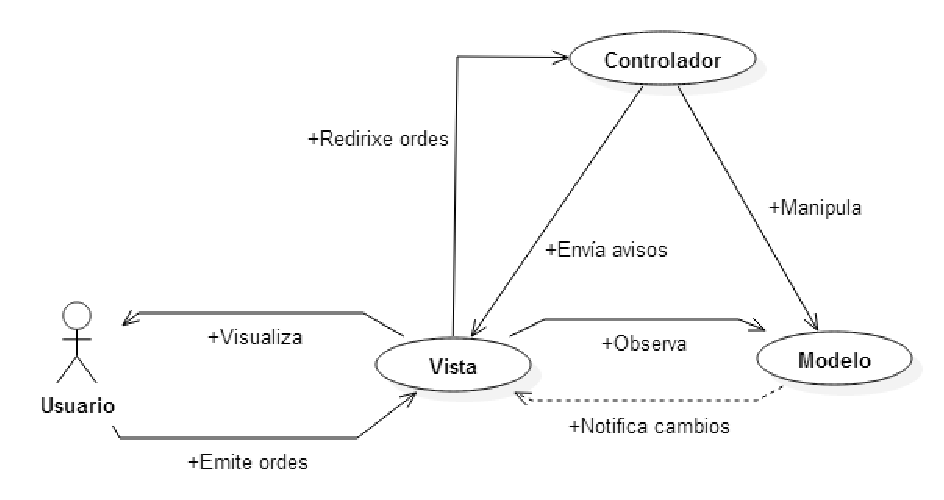
\includegraphics[width=\textwidth,height=\textheight,keepaspectratio]{figuras/MVC}
\caption{Modelo-Vista-Controlador para JDataMotion}
\label{MVC}
\end{figure}

As relacións marcadas cunha liña sólida son asociacións directas (unha clase que actúa de xeito explícito sobre os atributos ou métodos doutra), mentres que a relación marcada cunha liña descontinua representa unha relación indirecta (por exemplo, unha clase que resulta afectada pola actividade doutra). As relacións entre compoñentes detallaranse a continuación.

\begin{itemize}
\item O usuario emite ordes en forma de eventos cara a Vista ao interactuar cos seus botóns e menús.
\item A Vista identifica os eventos que recibe e redirixe cara o Controlador a orde asociada ao evento en cuestión.
\item O Controlador envía un aviso directo á Vista en caso de que a orde que recibe dela levase ao sistema a un estado de erro.
\item O Controlador manipula o Modelo segundo o contido da orde que recibe.
\item O Modelo actúa como entidade observada de cara á Vista. A Vista ten acceso ao Modelo para actualizar a súa aparencia.
\item Do mesmo xeito, que o Modelo sexa observado pola Vista implica que os cambios no modelo serán notificados á Vista, para que esta se actualice no momento do cambio.
\end{itemize} 

Imos documentar máis en profundidade a relación entre a Vista e o Modelo. Comentábamos que a Vista accede ao Modelo para actualizarse cando o desexe, pero ademais o Modelo, cando cambia, notifica á Vista o suceso deste cambio. Temos entón que a Vista actúa como entidade ``observadora'' dun Modelo que é a entidade ``observada''. En esencia, estamos definindo o patrón de deseño Observer.

O patrón de deseño Observer é a mellor resposta que podemos atopar a nivel de deseño para solucionar o problema de manter actualizados ao mesmo nivel o Modelo e a Vista. Se non botásemos man desta solución, teríamos dúas alternativas:

\begin{itemize}
\item Refrescar a vista cada certo intervalo tempo, o cal é ineficiente e seguiría permitindo a posibilidade de que se dese unha incoherencia Vista-Modelo entre refrescos.
\item Permitir ao Modelo que acceda directamente á Vista para invocar un método de actualización, é dicir, asociar directamente a Vista ao Modelo. Isto atenta contra a natureza do Modelo-Vista-Controlador, xa que o Modelo ten que almacenar a información do sistema e abstraerse por completo da Vista ou do módulo que se encargue de representar os seus contidos. Témonos que manter na premisa de que a Vista pode observar ao Modelo e acceder a el para ler datos, pero o Modelo non debe ser consciente da existencia de ningunha Vista.
\end{itemize} 

O patrón Observer pódese aplicar de forma moi sinxela ao noso proxecto. Basta con facer que a Vista implemente a interface \textit{Observer}, de xeito que a obrigue a implementar un método de actualización chamado \textit{update()}, que se disparará cando un obxecto observado cambie o seu estado. Por outra parte, o Modelo só necesita estender a clase \textit{Observable} para ser susceptible de ser observado por un \textit{Observer}. Ao estender esta clase, a Vista xa pode chamar ao método \textit{addObserver(Observer o)} do Modelo, pasándose a ela mesma como parámetro para así incluírse como observadora e ser notificada dos seus cambios.

A asociación dos patróns Modelo-Vista-Controlador e Observer baixo esta forma é bastante común. O libro Pattern-Oriented Software Architecture \cite{pattern-oriented-software-architecture} fai unha boa exposición do que acabamos de mencionar, e aporta o diagrama da figura \ref{MVC-observer} para sintetizar ambos patróns.

\begin{figure}
\centering
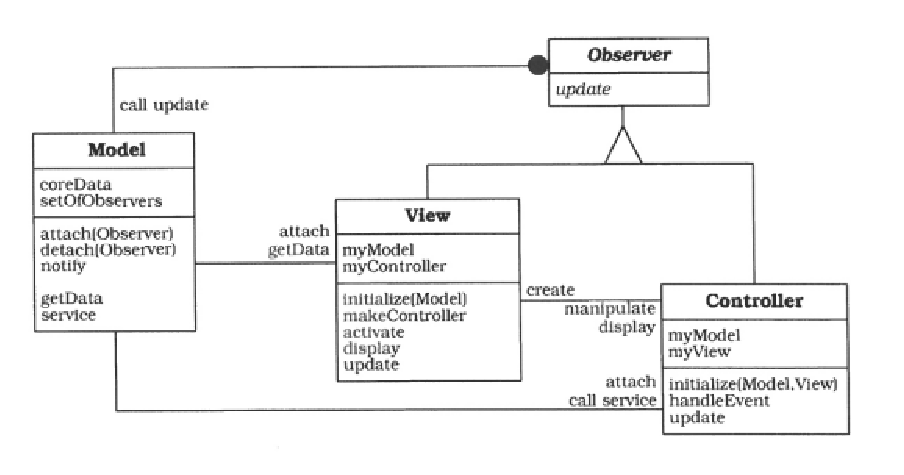
\includegraphics[width=\textwidth,height=\textheight,keepaspectratio]{figuras/MVC-observer}
\caption{Modelo-Vista-Controlador con Observer}
\label{MVC-observer}
\end{figure}

Probablemente a diferencia máis destacable que podemos atopar entre este diagrama e o diagrama que correspondería coa nosa aplicación sería que no noso caso só a Vista implementará a interface \textit{Observer}. O Controlador no noso proxecto non ten que actuar de ningún xeito especial ante os cambios do Modelo, xa que de feito el é o responsable directo deses cambios, e non necesita ser notificado das súas propias accións.
\cleardoublepage
\chapter{Exemplos}

\section{Un exemplo de sección}
Esta é {\it letra cursiva}, esta é {\bf letra negrilla}, esta é \underline{letra subrallada}, e esta é {\tt letra curier}. Letra {\tiny tiny}, {\scriptsize scriptsize}, {\small small}, {\large large}, {\Large Large}, {\LARGE LARGE} e moitas más. Exemplo de fórmula: $a=\int_o^\infty f(t)dt$.  E agora unha ecuación aparte:

\begin{equation}
S=\sum_{i=0}^{N-1} a_i^2 .
\label{mi_ecuacion}
\end{equation}

As ecuaciones se poden referenciar: ecuación (\ref{mi_ecuacion}).

\subsection{Un exemplo de subsección}
O texto vai aquí.
\subsection{Otro exemplo de subsección}
O texto vai aquí.
\subsubsection{Un exemplo de subsubsección}
O texto vai aquí.
\subsubsection{Un exemplo de subsubsección}
O texto vai aquí.
\subsubsection{Un exemplo de subsubsección}
O texto vai aquí.
\section{Exemplos de figuras e cadros}

A figura número \ref{enlace1}.

O cadro (taboa) número \ref{enlace2}.

\begin{figure}
\centerline{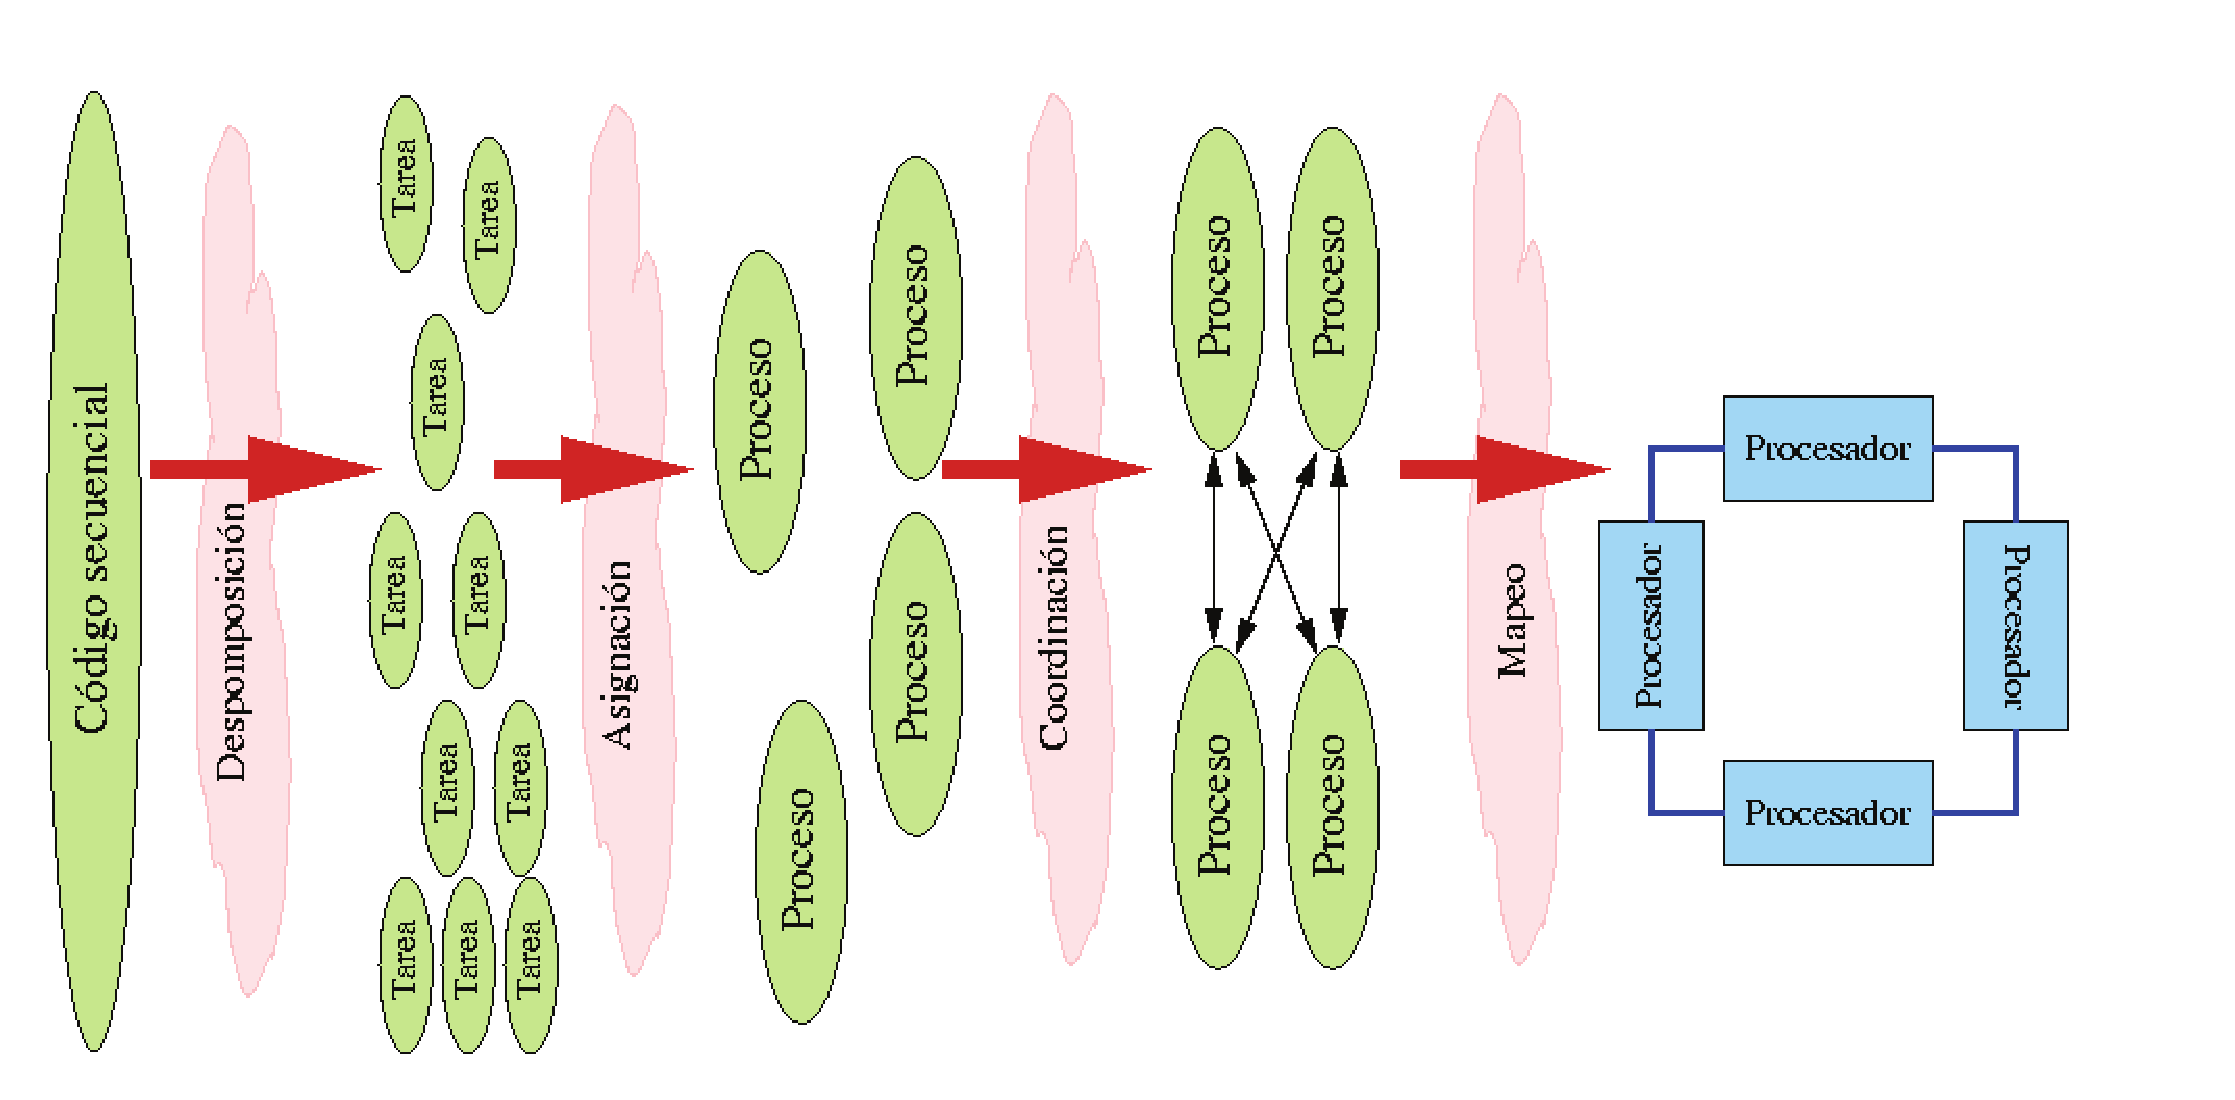
\includegraphics[width=15cm]{figuras/figura01.eps}}
\caption{Esta é a figura de tal e cal.}
\label{enlace1}
\end{figure}

\begin{table}
\begin{center}
\begin{tabular}{|l||r|c|} \hline
Izquierda & Derecha & Centrado  \\ \hline\hline
ll & r & cccc \\ \hline
llll & rrr & c \\ \hline
\end{tabular}
\caption{Esta é a táboa de tal e cal.}
\label{enlace2}
\end{center}
\end{table}

\section{Exemplos de referencias á bibliografía}
Este é un exemplo de referencia a un documento descargado da web \cite{cuda}. E este é un exemplo de referencia a unha páxina da wikipedia \cite{cdma}. Agora un libro \cite{gonzalez} e agora unha referencia a un artigo dunha revista \cite{patricia}. Tamén se poden pór varias referencias á vez \cite{cuda,gonzalez}.

\section{Exemplos de enumeracións}

Con puntos:

\begin{itemize}
\item Un.
\item Dous.
\item Tres.
\end{itemize}

Con números:

\begin{enumerate}
\item Catro.
\item Cinco.
\item Seis.
\end{enumerate}

Exemplo de texto verbatim:

\begin{verbatim}
O texto        verbatim 
     se visualiza tal
            como se escribe
\end{verbatim}

Exemplo de código C:

\lstset{language=C}

\begin{lstlisting}
#include <math.h>
main()
{  int i, j, a[10];
   for(i=0;i<=10;i++) a[i]=i; // comentario 1
   if(a[1]==0) j=1; /* comentario 2 */
   else j=2;
}
\end{lstlisting}

Exemplo de código Java:

\lstset{language=java}

\begin{lstlisting}
class HelloWorldApp {
    public static void main(String[] args) {
        System.out.println("Hello World!"); // Display the string.
    }
}
\end{lstlisting}



%
% Engadir os capitulos que fagan falta
%
\cleardoublepage
\chapter{Conclusións e posibles ampliacións}

Conclusións e posibles ampliacións


% Aquí empezan os apéndices
\appendix
\cleardoublepage
\chapter{Manuais técnicos}

Como xa mencionamos, o proxecto ofrece toda esta documentación, así coma o seu código fonte e referencias bibliográficas, a calquera persoa que teña intención de colaborar no desenvolvemento da aplicación.

Mención especial merece o contido da librería JDataMotion.common. Aquí os desenvolvedores dispostos a crear un filtro propio atoparán as clases e interfaces que deberán empregar. Para a implementación de filtros propios é mester ser capaz de manexar a clase Instances (estendida baixo InstancesComparable), e ser capaz de acceder e modificar as instancias e os atributos que almacena. Para isto, o propio subproxecto JDataMotion.common incorpora non só a API de programación de Weka, se non tamén os JavaDocs que describen cada clase e método da interface, e ademais inclúe o código fonte de toda a libraría. A integración dos JavaDocs na maioría dos IDEs facilitará a formación do desenvolvedor nos métodos e clases de Weka a medida que programa.

O desenvolvedor tamén dispón de métodos estáticos de interese estatístico dentro do proxecto común. Estes métodos traballan coas propias InstancesComparable, e poden ser de utilidade na implementación de novos filtros.

Para participar no desenvolvemento da propia aplicación JDataMotion aconséllase aproveitar a estrutura creada por Netbeans para abrir e continuar co proxecto. En calquera caso, a estrutura do programa é a seguinte:

\begin{description}
\item[/build:] \hfill
Contén as clases compiladas. Este directorio debe excluírse da xestión da configuración, pois depende do código que a orixina, o cal si é un elemento de configuración.
\item[/dist:] \hfill
Contén o arquivo JAR final, que podemos executar para arrancar a aplicación. Tamén se excluirá da xestión da configuración ao depender do código fonte.
\item[/filters:] \hfill
Contén unha copia de uso interno das librerías JAR importadas con filtros implementados. Tamén se excluirá da xestión da configuración, pois o seu contido depende da experiencia de cada usuario coa aplicación.
\item[/lib:] \hfill
Contén as librerías e demais dependencias da aplicación. Si constitúe un elemento de configuración.
\item[/nbproject:] \hfill
Carpeta na que NetBeans garda a súa configuración con respecto ao programa. Si constitúe un elemento de configuración.
\item[/src:] \hfill
Contén todo o código fonte da aplicación, nunha xerarquía de carpetas que representa os paquetes. Si constitúe un elemento de configuración.
\item[/store:] \hfill
Contén un JAR autocontido da aplicación, é dicir, que xa conta con todas as dependencias integradas. Excluirase da xestión da configuración, xa que depende do código fonte e das librerías, e ambos son xa elementos de configuración.
\item[/test:] \hfill
Contén todo o código fonte das probas da aplicación, nunha xerarquía de carpetas que representa os paquetes. Si constitúe un elemento de configuración.
\item[.gitignore:] \hfill
Ficheiro cunha liña por cada directorio ou ficheiro que deba ser excluído da xestión da configuración. Si constitúe un elemento de configuración en si mesmo.
\item[build.xml:] \hfill
Ficheiro que usa NetBeans para compilar, executar ou realizar outras accións sobre este proxecto. Si constitúe un elemento de configuración.
\item[configuracion.properties:] \hfill
Contén a configuración de usuario almacenada. Tamén se excluirá da xestión da configuración, pois o seu contido depende da experiencia de cada usuario coa aplicación.
\item[manifest.mf:] \hfill
Ficheiro de configuración da extensión e do paquete. Si constitúe un elemento de configuración.
\item[run.bat:] \hfill
Script de arranque para plataformas Windows. Si constitúe un elemento de configuración.
\item[run.sh:] \hfill
Script de arranque para plataformas Linux. Si constitúe un elemento de configuración.
\end{description}
 
\cleardoublepage
\chapter{Manuais de usuario}

Manuais de usuario: incluirán toda a información precisa para aquelas persoas que utilicen o Sistema: instalación, utilización, configuración, mensaxes de erro, etc. A documentación do usuario debe ser autocontida, é dicir, para o seu entendemento o usuario final non debe precisar da lectura de outro manual técnico.

\cleardoublepage
\chapter{Licenza}
Se se quere pór unha licenza (GNU GPL, Creative Commons, etc), o texto da licenza vai aquí.


\cleardoublepage
\markboth{BIBLIOGRAFÍA}{BIBLIOGRAFÍA}
\addcontentsline{toc}{chapter}{Bibliografía}


\begin{thebibliography}{99}

\bibitem{weka} Weka 3 - Data Mining with Open Source Machine Learning Software in Java. Sitio web {\it http://www.cs.waikato.ac.nz/ml/weka/}.

\bibitem{jfreechart} Proxecto JFreeChart. Sitio web {\it http://www.jfree.org/jfreechart}.

\bibitem{arff} Formato de Archivo Atributo-Relación (ARFF). Información dispoñible en {\it http://www.cs.waikato.ac.nz/ml/weka/arff.html} [Última consulta: 10/07/2015].

\bibitem{java} Java. Sitio web {\it https://www.java.com/en/}.

\bibitem{preciokWh_espana} Tarifasgasluz. Precio del kWh en España. Sitio web {\it http://www.endesaonline.com/es/empresas/dual/empresas/4/precios/index.asp} [Última consulta: 10/07/2015].

\bibitem{energyusecalculator} Electricity usage of a Laptop or Notebook. Sitio web {\it http://energyusecalculator.com/electricity\_laptop.htm} [Última consulta: 10/07/2015].

\bibitem{scrum} Scrum. Definicións extraídas de {\it http://es.wikipedia.org/wiki/Scrum} [Última consulta: 10/07/2015].

\bibitem{acunote} Acunote. Sitio web {\it http://www.acunote.com/}.

\bibitem{github} GitHub. Sitio web {\it https://github.com/}.

\bibitem{junit} JUnit. Sitio web {\it http://junit.org/}.

\bibitem{lumzy} Lumzy. Sitio web {\it http://www.lumzy.com/}.

\bibitem{ieee-std-830-1998} IEEE-STD-830-1998: Especificaciones de los requisitos del software. Ler máis {\it http://www.ctr.unican.es/asignaturas/is1/IEEE830\_esp.pdf} [Última consulta: 10/07/2015].

\bibitem{pattern-oriented-software-architecture} Buschmann, Frank. 1996. \textit{Pattern-Oriented Software Architecture Volume 1: A System of Patterns}. Wiley. 

\end{thebibliography}


\cleardoublepage
\pagestyle{plain}
\chapter*{Glosario}
\begin{description}
  \item[Sesión] \hfill
  Interacción co sistema e as súas funcionalidades. Inclúe a importación duns datos, o seu procesado, filtrado e visualización.
  \item[Experimento] \hfill
  Ver sesión.
	\item[Diagrama de dispersión] \hfill
  Diagrama matemático que fai uso das coordenadas cartesianas para amosar os valores de dúas variables para un conxunto de datos. Cada punto no diagrama referencia un valor ao longo do eixo de ordenadas e outro ao longo do eixo de abscisas.
	\item[Modelo] \hfill
  Estrutura e contido dos datos cos que se traballa no experimento. Abrangue tanto os tipos dos atributos coma os seus valores dentro de cada entrada, así coma o nome do conxunto de datos, ou a marca do atributo que actúa de índice temporal.
	\item[Filtro] \hfill
  Ferramenta configurable que en función dos seus parámetros pode converter, a partir dun modelo A de entrada, un modelo B de saída.
	\item[Visualización] \hfill
  Presentación gráfica da relación, neste caso baixo a forma de diagramas de dispersión.
	\item[Reprodución] \hfill
  Activación dunha visualización para que cambie o seu estado ao longo do tempo, neste caso en función dun índice ou variable temporal.
	\item[Índice temporal] \hfill
  Atributo do modelo que representa a orde na que os datos foron tomados, foron detectados, queren ser priorizados ou simplemente se desexan amosar. Se non se define, asúmese como índice temporal a orde das entradas do modelo.
	\item[Entrada] \hfill
  Ver instancia.
	\item[Instancia] \hfill
  Vector de datos que contén un valor para cada atributo do modelo. Pode conter valores nulos.
	\item[Atributo] \hfill
  Cada unha das variables coas que traballa o modelo.
	\item[Atributo numérico] \hfill
  Atributo que só pode tomar valores numéricos.
	\item[Atributo de tipo data] \hfill
  Atributo que só pode tomar valores de tipo data.
	\item[Atributo de tipo string] \hfill
  Atributo que pode tomar calquera valor en forma de cadea de caracteres.
	\item[Atributo nominal] \hfill
  Atributo que só pode tomar unha serie de valores concretos.
	\item[Relación] \hfill
 Ver modelo.
\item[Reprodución] \hfill
 Visualización dinámica da relación, é dicir, presentación dunha relación na que cada entrada se visualiza nun momento do tempo determinado.
\item[Scatterplot] \hfill
 Diagrama de dispersión.
\item[Comando] \hfill
 Entidade que representa unha orde para o sistema. Contén información sobre o artefacto ao que afecta, o tipo de orde que se expresa e os parámetros necesarios para a súa execución.
\end{description}

\end{document}
